%%% template.tex
%%%
%%% This LaTeX source document can be used as the basis for your technical
%%% paper or abstract. Intentionally stripped of annotation, the parameters
%%% and commands should be adjusted for your particular paper - title, 
%%% author, article DOI, etc.
%%% The accompanying ``template.annotated.tex'' provides copious annotation
%%% for the commands and parameters found in the source document. (The code
%%% is identical in ``template.tex'' and ``template.annotated.tex.'')

\documentclass[]{acmsiggraph}
\usepackage{algorithm}
\usepackage[noend]{algpseudocode}
\TOGonlineid{45678}
\TOGvolume{0}
\TOGnumber{0}
\TOGarticleDOI{0}
\TOGprojectURL{}
\TOGvideoURL{}
\TOGdataURL{}
\TOGcodeURL{}
\usepackage{color}
%\definecolor{red}{rgb}{0.9, 0.17, 0.31}
\usepackage{multirow}
\usepackage{subfig}
\usepackage{xcolor}
\usepackage{lipsum}
\usepackage{listings}
\usepackage{graphicx}
\usepackage{glsllst} % My own package providing markup listing for glsl
\usepackage{rmlst}   % My own package providing markup listing for renderman
\usepackage{amsmath}
\usepackage{hyperref}

\lstset{
	backgroundcolor=\color[rgb]{0.95, 0.95, 0.95},
	tabsize=3,
	%rulecolor=,
	basicstyle=\footnotesize\ttfamily,
	upquote=true,
	aboveskip={1.5\baselineskip},
	columns=fixed,
	showstringspaces=false,
	extendedchars=true,
	breaklines=true,
	prebreak = \raisebox{0ex}[0ex][0ex]{\ensuremath{\hookleftarrow}},
	frame=none,
	aboveskip=15pt,
	belowskip=8pt,
	captionpos=t,
	showtabs=false,
	showspaces=false,
	showstringspaces=false,
	identifierstyle=\ttfamily,
	%keywordstyle=\color{red}\bfseries,
	%keywordstyle=[1]\bfseries\color{syntaxBlue},
	%keywordstyle=[2]\bfseries\color{syntaxRed},
	%keywordstyle=[3]\color{blue}\bfseries,
	%keywordstyle=[4]\bfseries\color{syntaxBlue},
	commentstyle=\color[rgb]{0.082,0.639,0.082},
	keywordstyle=[1]\bfseries\color[rgb]{0,0,0.75},
	keywordstyle=[2]\bfseries\color[rgb]{0.5,0.0,0.0},
	keywordstyle=[3]\bfseries\color[rgb]{0.127,0.427,0.514},
	keywordstyle=[4]\bfseries\color[rgb]{0.4,0.4,0.4},
	stringstyle=\color[rgb]{0.639,0.082,0.082},
}

\usepackage{listings}

% \setlength{\parindent}{4em}
\setlength{\parskip}{0.5em}

\title{\texttt{sonipy}: A Perceptually Uniform Sonification Package}

\author{Locke Patton \textsuperscript{123}, Emily Levesque \textsuperscript{14}}
% \pdfauthor{Richard Southern}

\keywords{sonification}

\begin{document}

\teaser{
    \centering
    
    \vspace{-\baselineskip}
    \scriptsize  \textsuperscript{1}Department of Astronomy, University of Washington, Seattle, WA 98195 USA\\
    \textsuperscript{2}Harvard-Smithsonian Center for Astrophysics, 60 Garden St, Cambridge, MA 02138
    \normalsize

    \vspace{\baselineskip}
    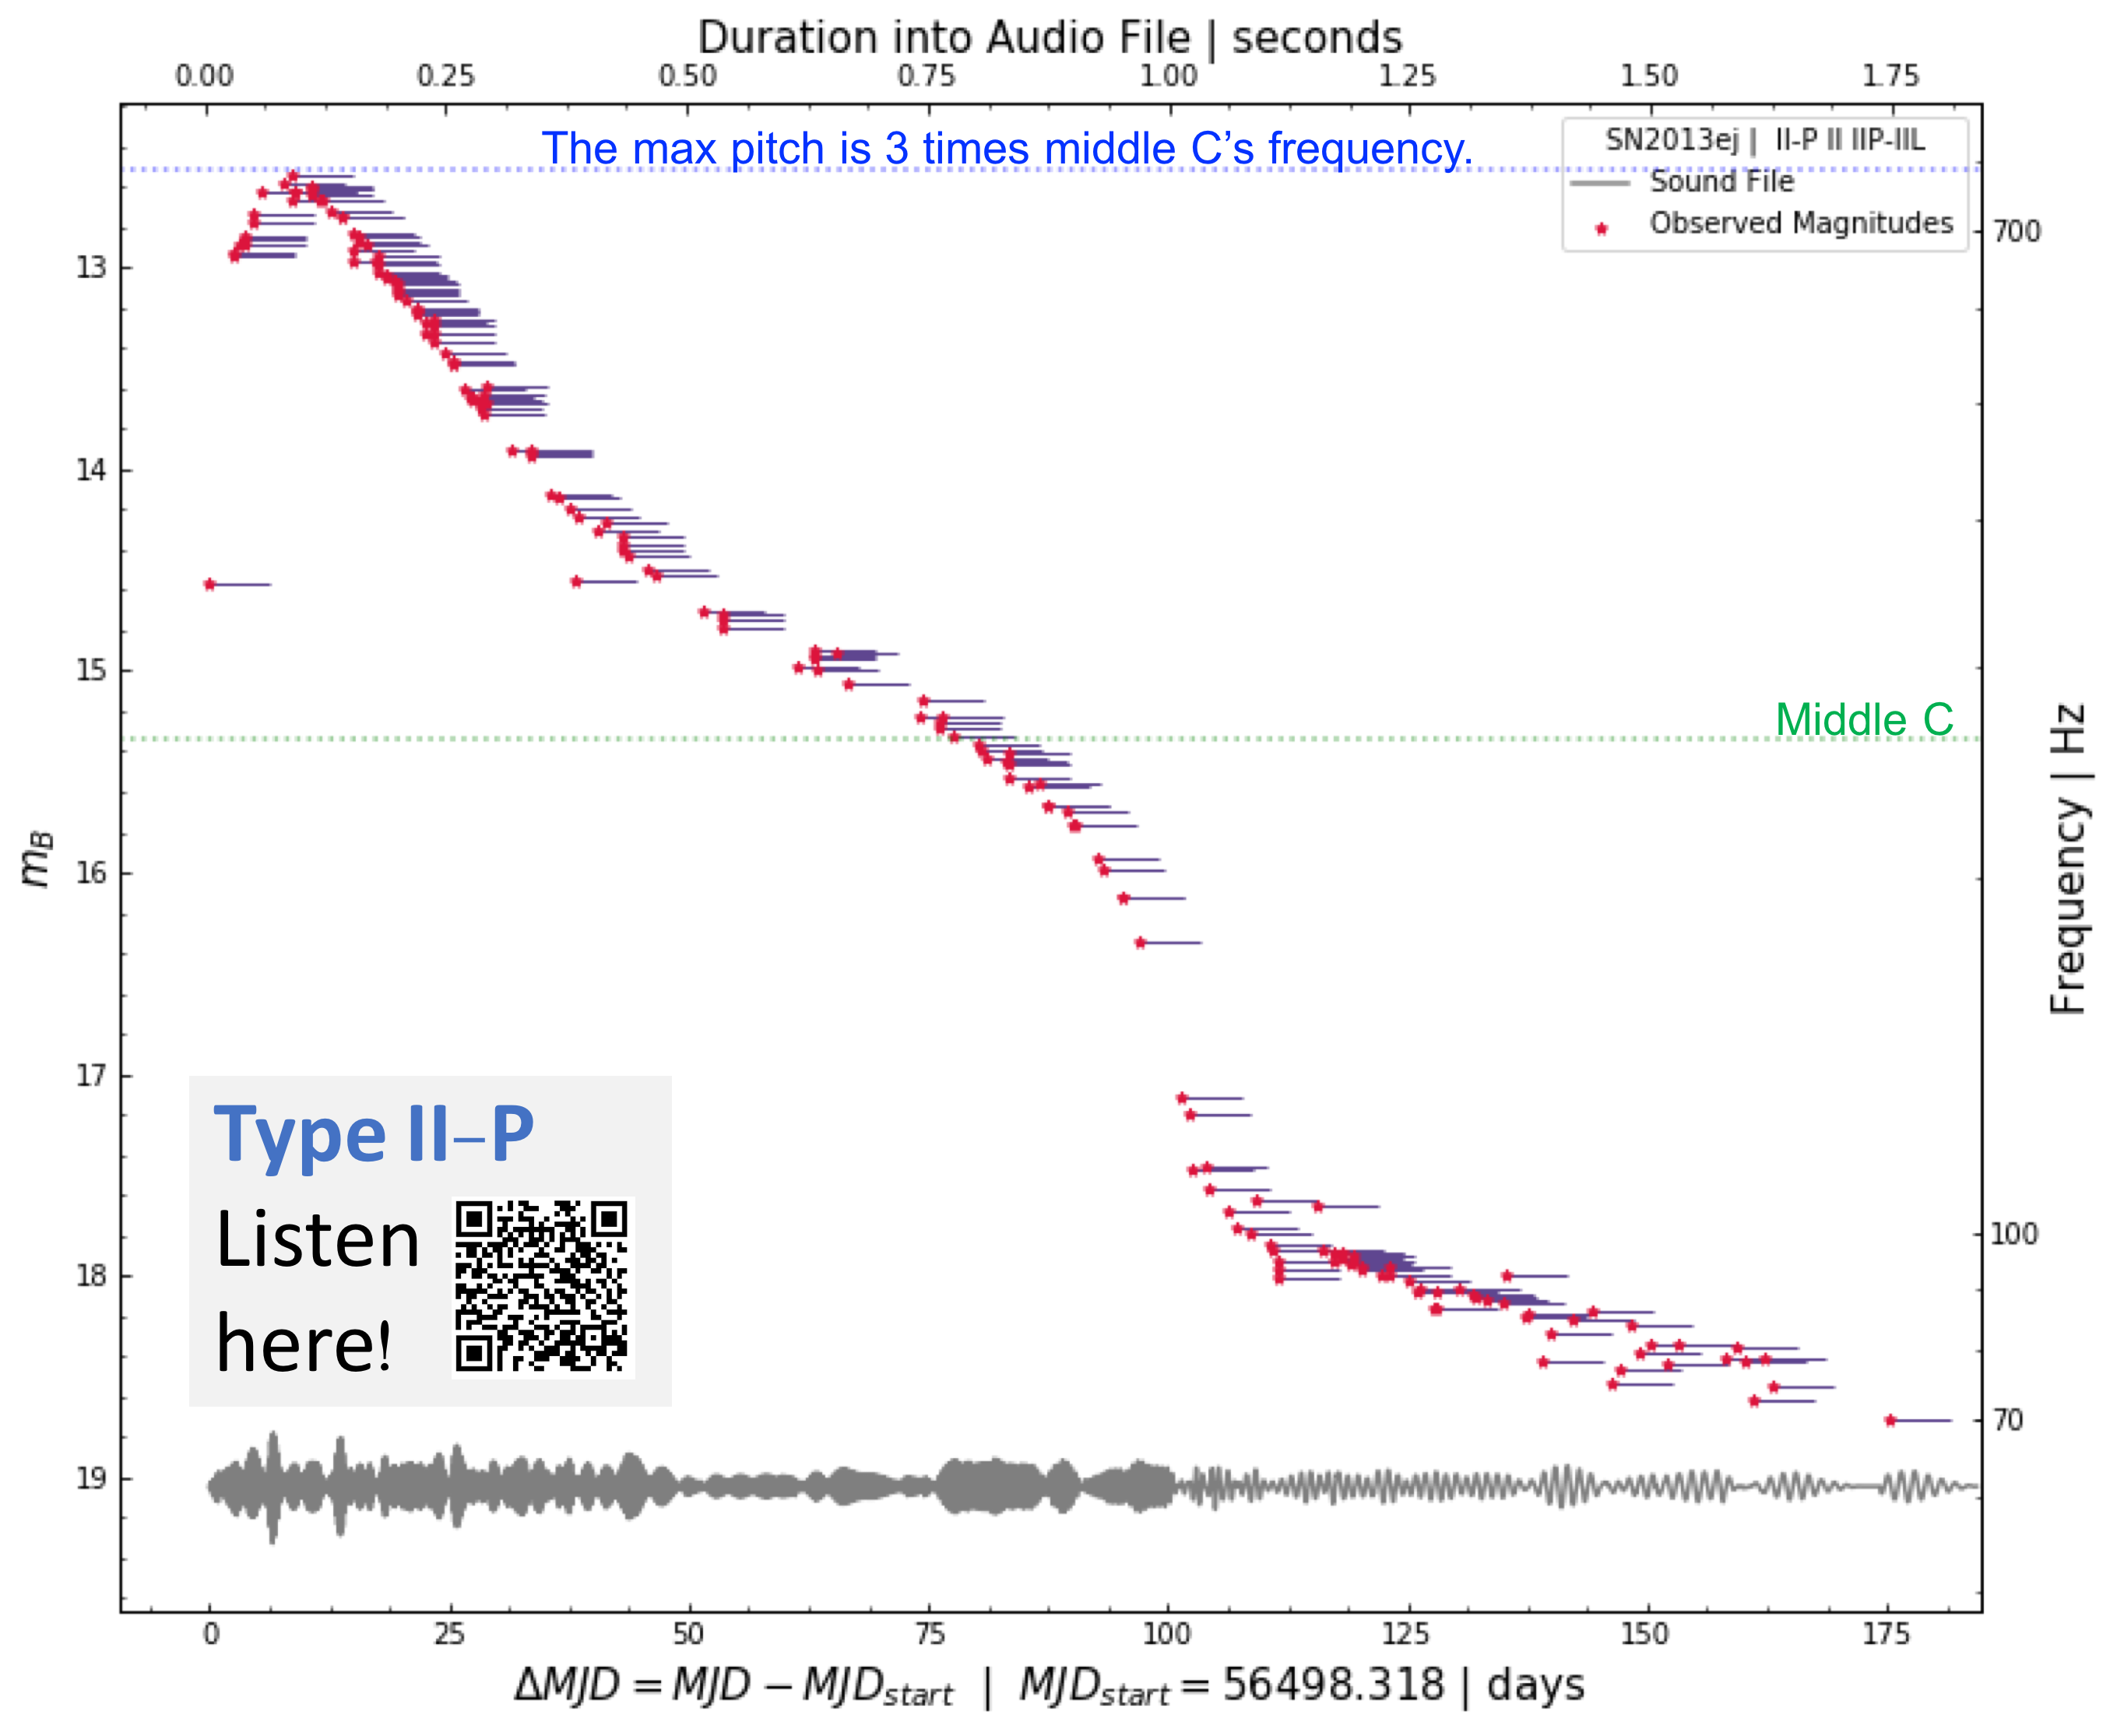
\includegraphics[width=.65\linewidth]{paper/images/Picture1-nobkgd.png}
    \captionsetup{width=.65\linewidth}
    \caption{Example sonification case: an exploding star's change in brightness is plotted against time. Each datapoint corresponds to a tone blip at a frequency specified by its y value and a time specified by its x value. As the sound file plays, it scans the plot left to right, with the brightest moments of the exploding star reaching pitches of 3 times middle C on the piano and the tail of the cooling supernovae remnant dropping into lower audible pitches.}
}


\maketitle
\footnotetext[3]{locke.patton@cfa.harvard.edu}
\footnotetext[4]{emsque@uw.edu}

\section{Introduction} \label{sec:introduction}

\texttt{Sonipy} moves beyond visual analyses by sonifying scatter-plot data, producing audio files that depict variations in y as perceptually uniform changes in pitch. Blips are sounded in time at intervals corresponding to x values.

\subsection{Understanding pitch}
The cent is a logarithmic unit of measure for pitch intervals where $n \approx 3986\log(b/a)$ defines the number of cents between the pitch frequencies a and b.

\subsection{Human Pitch Sensitivity}
The average person is capable of discerning independent subsequent pitches with a difference of ~10 cents (Kollmeier et al. 2008). The human ear is most sensitive to frequencies between ~ 500-4000 Hz, similar to the range of a standard piano.

With these parameters, xy scatterplot data can be translated into audio files that map y values to specific pitch frequencies, with the minimum discernible $\Delta y$ corresponding to a 10 cent pitch difference.

\section{The Case for Sonification}

\subsection{Why sonify lightcurves?}

Thanks to the nature of human hearing, we can audibly discern pitch differences of 10 cents. On a y scale ranging from 0 to 10, that corresponds to hearing variations as small as $\Delta y~0.03$. This simultaneous depth and range of pitch is unique to sound and incredibly powerful as a tool for understanding nuances in data.

Furthermore, through our sonification efforts of periodically variable astronomy sources, we have discovered that periodicity that is visually indiscernible can be heard in our sonified data.

Finally and most importantly, this approach opens up science and citizen science to participants who are visually impaired, and empowers BVI individuals to explore their own data.

% At this scale we can “hear” lightcurves that span up to 10 magnitudes. 

\section{Our Sonification Technique}
% NON COMPLETE

\begin{multline}\label{eq:kajiya}
L_o \left( \mathbf{x},\omega_o,\lambda,t \right) = L_e\left(\mathbf{x},\omega_o,\lambda,t \right) + \\
   \int_\Omega f_r \left(\mathbf{x},\omega_i,\omega_o,\lambda,t\right) L_i\left(\mathbf{x},\omega_i,\lambda,t\right) \left(\omega_i \cdot \mathbf{n}\right) d\omega_i
\end{multline}

\begin{figure}[h]
\centering
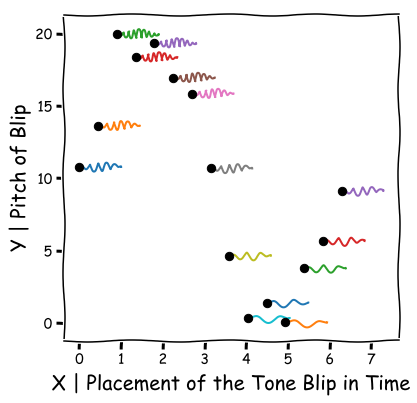
\includegraphics[width=.7\linewidth]{paper/images/Method1.png}
\end{figure}

\begin{enumerate}
\item Each data point corresponds to a short tone in the sound file.
\item X value determines the placement of the tone in time.
\item The Y value determines the tone’s pitch.
\item As Y value decreases, the tone’s pitch gets lower.
\end{enumerate}


\subsection{Why this method? }

Each datapoint corresponds to a tone blip at a frequency specified by its y value and a time specified by its x value. As the sound file plays, it scans the plot left to right, with higher y datapoints causing higher pitched blips and vica verca.

Our method is tailored to the capabilities of the human ear and audio equipment. It is flexible, applies to a broad variety of data inputs, is fast to generate, and offers a unique means of classifying data.

We avoid methods that match changes in y to decibels, because our perception of loudness is not a perceptually uniform space and inconsistent across users. As our method is tailored to a science case, a linear increase in y corresponds to a perceptually uniform and linear increase in perceived pitch.

\section{The Code}
% NON COMPLETE

\textbf{Total File Duration: } Duration is set by a total time, a duration scale, or by choosing the length of minimum or maximum time difference.

\textbf{Frequency scale:} Frequency is set by one of the following: a frequency minimum and maximum, or a frequency maximum and a cents / y value scale value.

\vspace{-1.25\baselineskip}
\begin{lstlisting}[language=Python, frame=lines,label={lst:code_direct}, caption={A simple textured shader.}, basicstyle=\footnotesize]
from sonify import *

C4 = 261.6 # Hz
args = {'frequency_min' : C4,
        'frequency_max' : C4*4,
        'value_min' : 0,
        'value_max' : 1}

SN = MultiTone(values=x, durations=y,
               length=0.5, **args)
SN.SaveTone()
\end{lstlisting}

\section{Our Astronomy Case Study}
\subsection{Citizen Science - Supernova Lightcurves}
We’re building TransientZoo, a citizen science program that will allow participants, including the visually impaired, to classify supernova lightcurves using sound.

Figure \ref{fig:Ia} and \ref{fig:IIb} are two examples of successfully sonified audio light curves, for a Type IIb and Type Ia supernova. We find that linear and plateau supernova light curves can be audibly differentiated. This approach offers a new tool for citizen science lightcurve classification.


\begin{figure}[h]
\centering
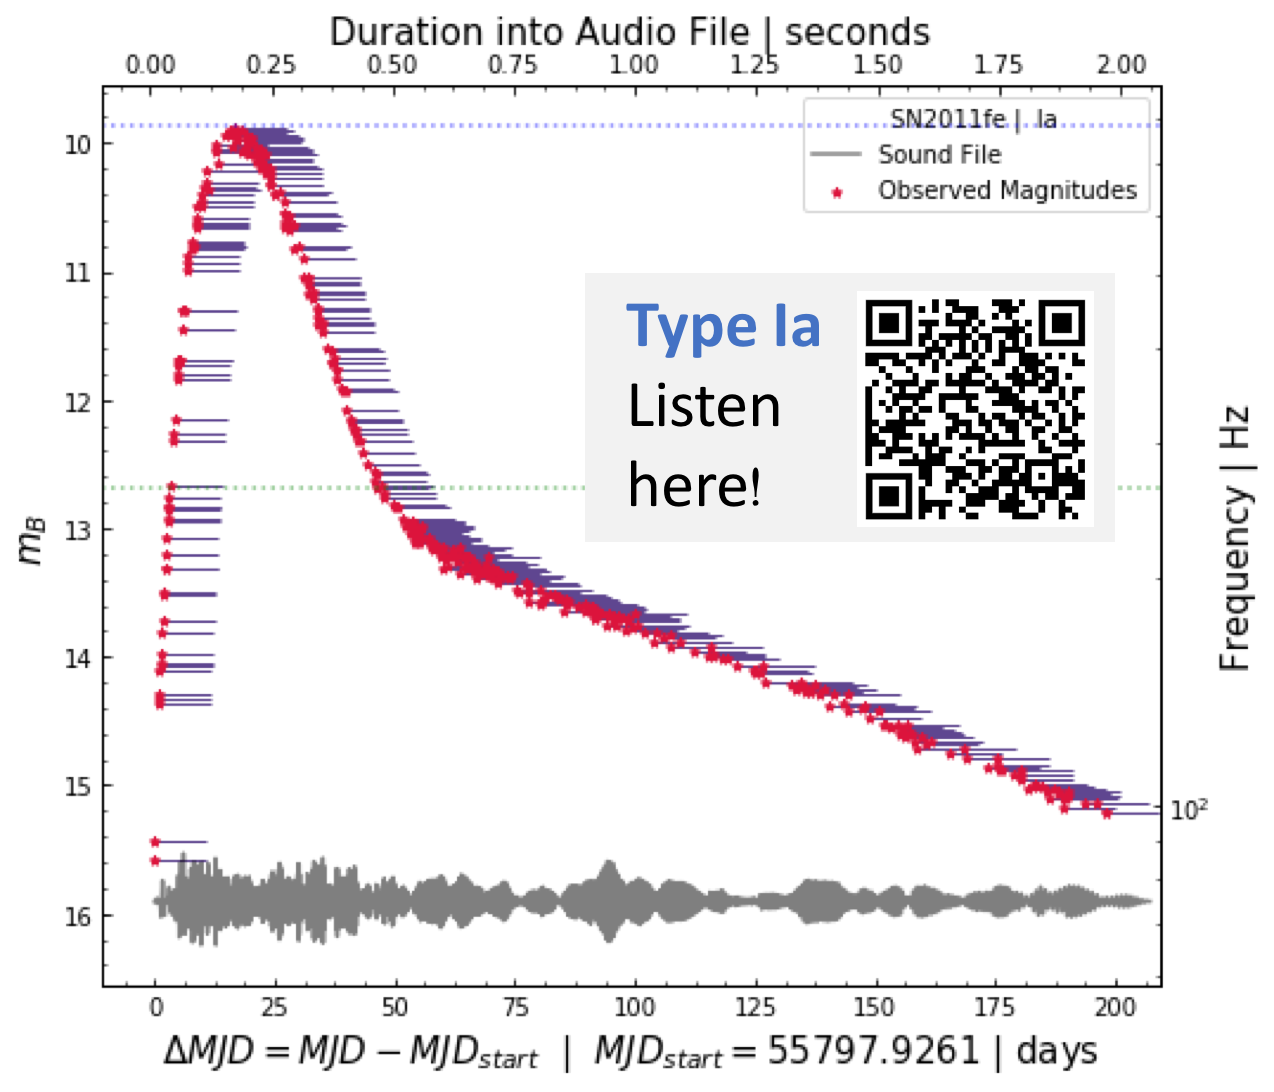
\includegraphics[width=.7\linewidth]{paper/images/Ia.png}
\caption{A type Ia supernova lightcurve.}
\label{fig:Ia}
\end{figure}

\begin{figure}[h]
\centering
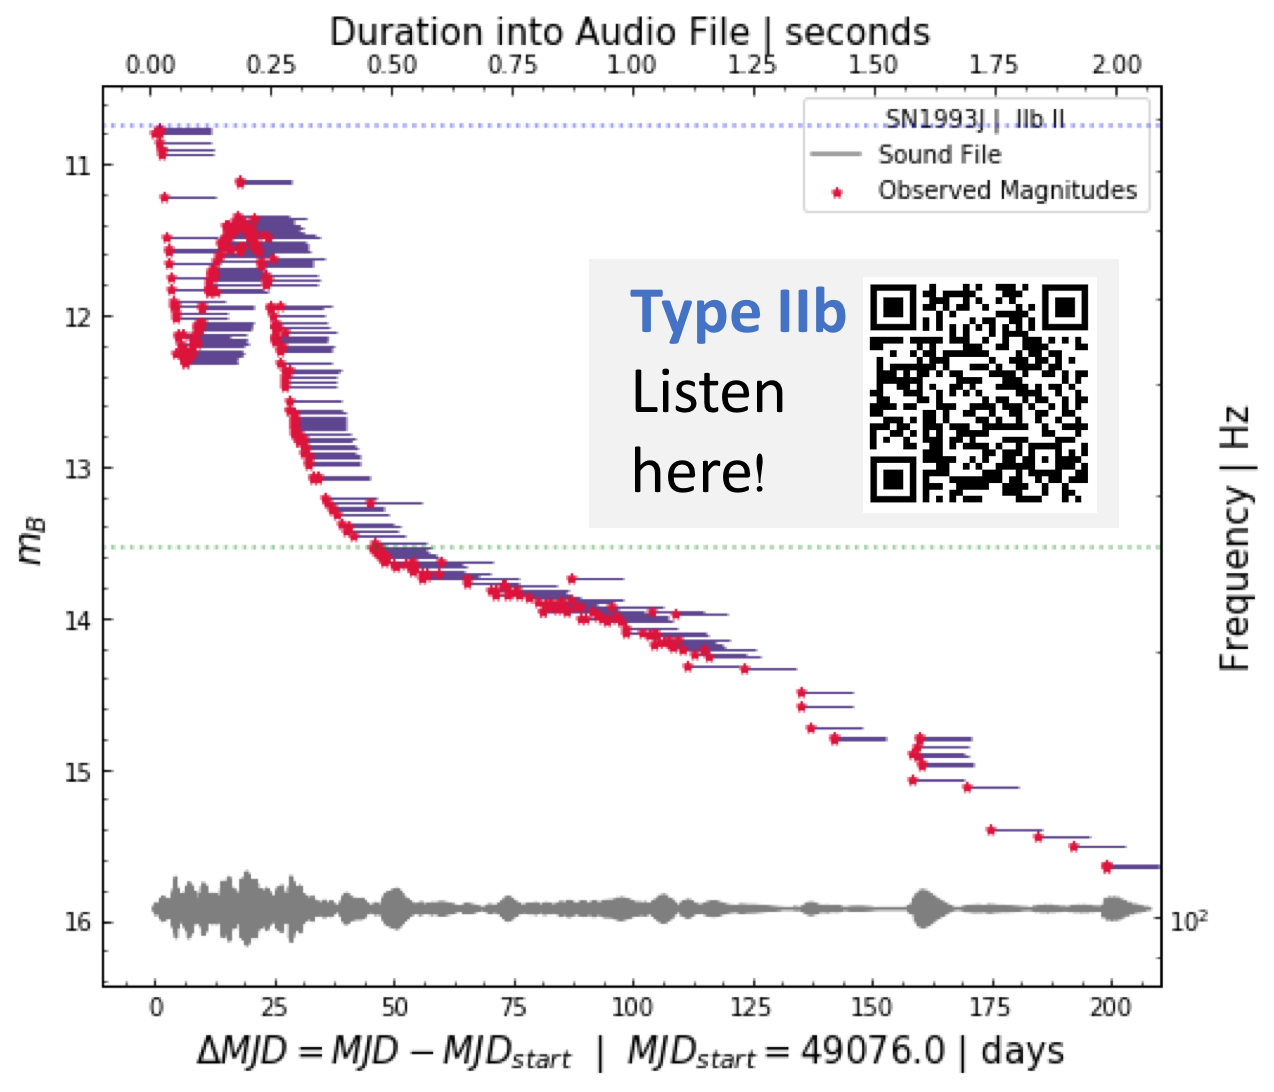
\includegraphics[width=.7\linewidth]{paper/images/IIb.png}
\caption{A type IIb supernova lightcurve.}
\label{fig:IIb}
\end{figure}

\subsection{Other Variable Objects in Astronomy}
We’ve also explored the sonification of other time-domain data, which will eventually help TransientZoo expand into LightcurveZoo.To the right are pictured examples of an eclipsing binary from Kepler’s catalogue and an RR Lyrae from our observations. LightcurveZoo will ultimately include a collection of transients: supernovae, binaries, and variable stars.

% \begin{figure}
% \centering
% 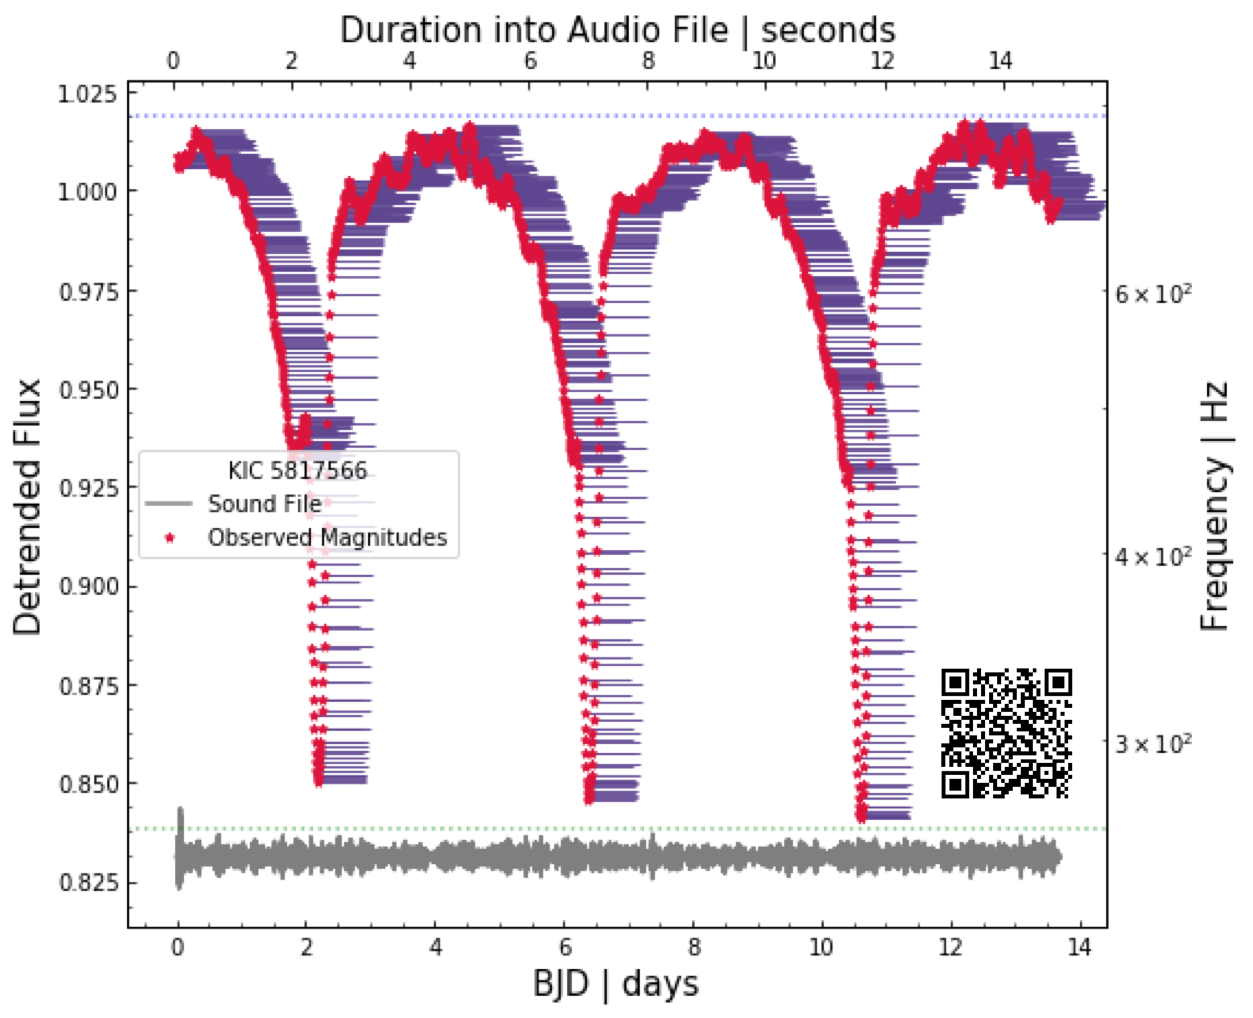
\includegraphics[width=.7\linewidth]{paper/images/EB.png}
% \caption{An eclipsing stellar binary.}
% \label{fig:EB}
% \end{figure}

% \begin{figure}
% \centering
% 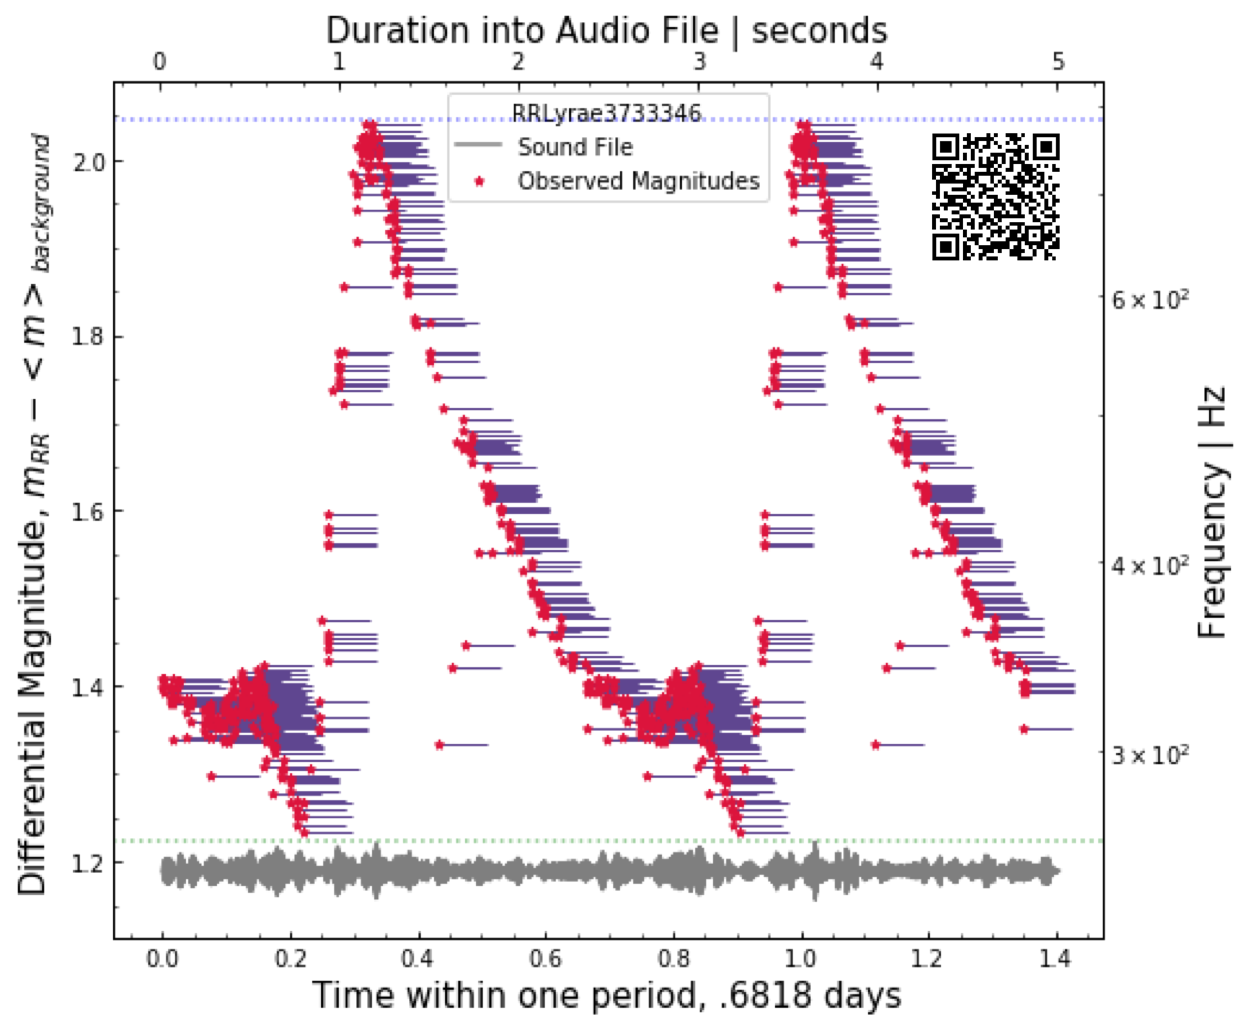
\includegraphics[width=.7\linewidth]{paper/images/RRLyrae.png}
% \caption{A variable star, phased over it's period.}
% \label{fig:RRLyrae}
% \end{figure}

\end{document}